%%%%%%%%%%%%%%%%%%%%%%%%%%%%%%%%%%%%%%%%%%%%%%%%%%%%%%%%%%%%%%%%%%%%%%%%%%%

\documentclass{standalone}

\usepackage{mathptmx}
\usepackage{tikz}
\usetikzlibrary{external}
\tikzexternalize{square-inscribed-circle}

%% We default to Times.
\renewcommand{\rmdefault}{ptm}
\renewcommand{\ttdefault}{pcr}
%% Enable Times/Palatino main text font.
\normalfont\selectfont

\newcommand{\comma}{,\,}
\newcommand{\tuple}[2]{\left({#1}\comma {#2}\right)}

%% Draw a point and label it.
%%
%% #1 -- Coordinates of the point.
%% #2 -- Label the point with this name.
%% #3 -- Where to place the label.
\newcommand{\xyPoint}[3]{%%
  \node[nodeStyle] at (#1) {};
  \node[#3] at (#1) {$#2$};
}

%%%%%%%%%%%%%%%%%%%%%%%%%%%%%%%%%%%%%%%%%%%%%%%%%%%%%%%%%%%%%%%%%%%%%%%%%%%
%% A circle inscribed inside a square.
%%%%%%%%%%%%%%%%%%%%%%%%%%%%%%%%%%%%%%%%%%%%%%%%%%%%%%%%%%%%%%%%%%%%%%%%%%%

\begin{document}

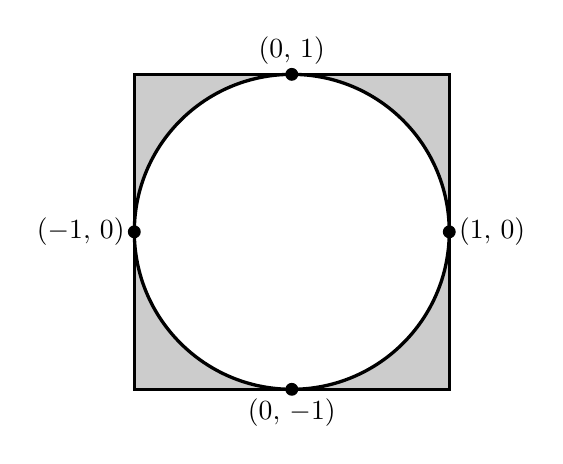
\begin{tikzpicture}[%%
  circleStyle/.style={-,very thick,fill=white},%%
  nodeStyle/.style={draw,inner sep=1.5pt,circle,fill=black,black},%%
  squareStyle/.style={-,very thick,fill=gray!40}%%
]
%%
%%
\pgfmathsetmacro{\radius}{2}
\pgfmathsetmacro{\xlow}{0}
\pgfmathsetmacro{\ylow}{0}
%%
\coordinate (centre) at (\xlow,\ylow);
\coordinate (lowerLeft) at (\xlow-\radius,\ylow-\radius);
\coordinate (upperRight) at (\xlow+\radius,\ylow+\radius);
%% Points on the circle.
\coordinate (pbottom) at (\xlow,\ylow-\radius);
\coordinate (pleft) at (\xlow-\radius,\ylow);
\coordinate (pright) at (\xlow+\radius,\ylow);
\coordinate (ptop) at (\xlow,\ylow+\radius);
%%
%%
%% The square.
\draw[squareStyle] (lowerLeft) rectangle (upperRight);
%% The circle.
\draw[circleStyle] (centre) circle[radius=\radius];
%% Some points on the circle.
\xyPoint{pright}{\tuple{1}{0}}{right}
\xyPoint{pleft}{\tuple{-1}{0}}{left}
\xyPoint{ptop}{\tuple{0}{1}}{above}
\xyPoint{pbottom}{\tuple{0}{-1}}{below}
\end{tikzpicture}

\end{document}
